\documentclass{article}
%\usepackage{geometry}
%\geometry{top = 1in, bottom = 1in, left = 1in, right = 1in}
\usepackage[top = 0.7in, bottom = 0.7in, left = 0.7in, right = 0.7in]{geometry}
\usepackage{amsmath,amssymb,amsthm,mathrsfs}
\usepackage{graphicx}
\usepackage{bm}
\usepackage{float}
\usepackage[font=footnotesize,labelfont=bf]{caption}
\usepackage{movie15}
\usepackage{hyperref}

\usepackage{fancyhdr}
\pagestyle{fancy}
\rhead{\footnotesize {08/28/2012 ; MESA version 4411} }
\chead{\footnotesize {Authors: Jared Brooks, Lars Bildsten, Bill Paxton} }
\lhead{\footnotesize {mesa/star/test\_suite/low\_z} }

\begin{document}
	
	\begin{center}
	  \begin{Large}
	    \textbf{LOW Z}\\
	  \end{Large}
	\end{center}

        This test is to show the evolution of a 0.8 $M_\odot$ low metallicity ($Z=10^{-4}$) star from the pre-main sequence to the main sequence.  The run should be cut off when the effective temperature reaches 6600 K (\texttt{Teff\_upper\_limit = 6600}).\\

        The HR-diagram below (figure \ref{fig:1}) shows the Hayashi track and the beginning of the main sequence, starting in the upper right corner.

        \begin{figure}[H]
          \centering
          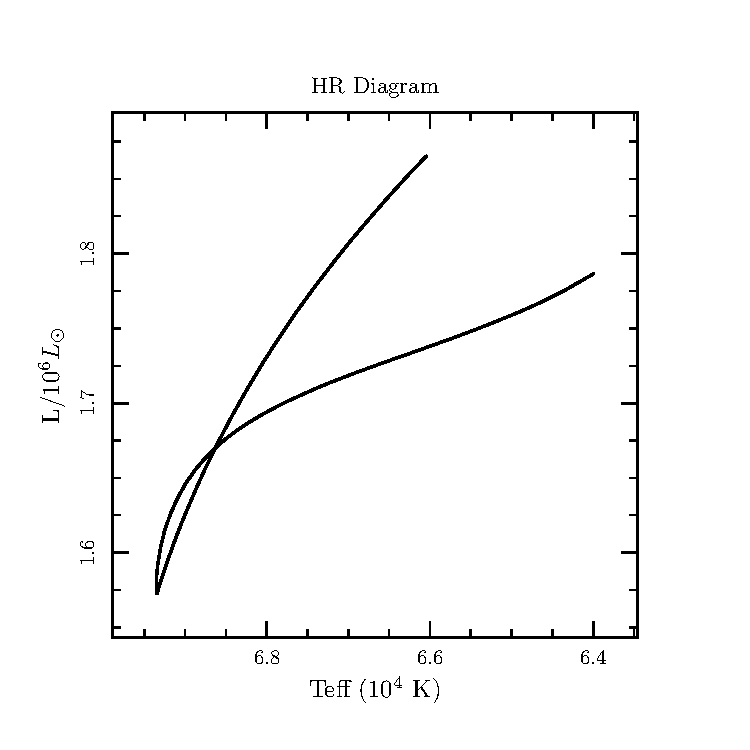
\includegraphics[width = 5in]{/Users/jaredbrooks/low_z/plots_out/HR_Diagram.pdf}
          \caption{HR-diagram, evolution start in upper right corner}
          \label{fig:1}
        \end{figure}

        \pagebreak

        The two abundance profiles below taken from the start (figure \ref{fig:2}) and the end (figure \ref{fig:3}) of the run show that the abundances in the envelope change very little, and that hydrogen in the core is being consumed.

        \begin{figure}[H]
          \begin{minipage}[b]{0.5\linewidth}
	    \centering
	    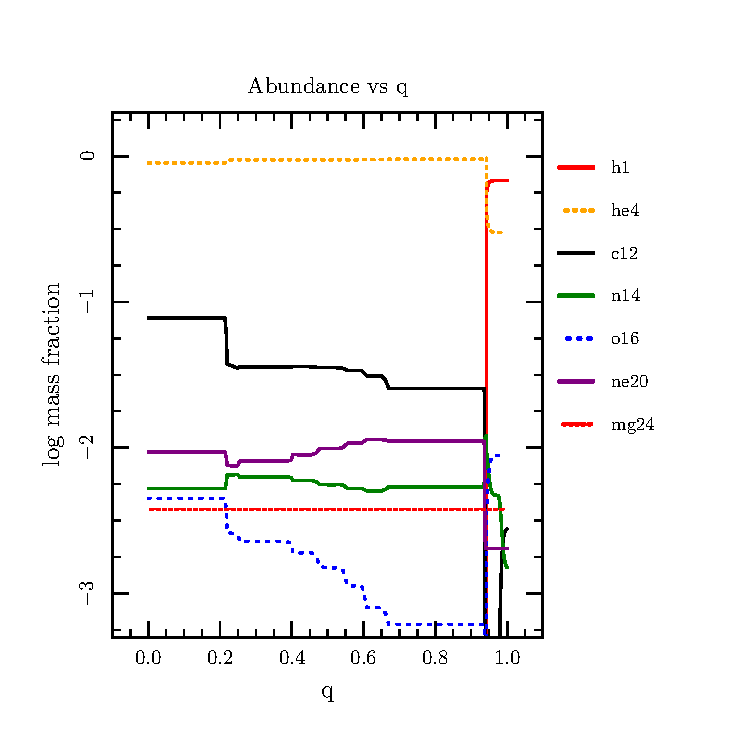
\includegraphics[width = 3.8in]{/Users/jaredbrooks/low_z/plots_out/Abundance_vs_q_1.pdf}
	    \caption{Abundance profile at start of run}
	    \label{fig:2}
          \end{minipage}
          \hspace{0cm}
          \begin{minipage}[b]{0.5\linewidth}
            \centering
            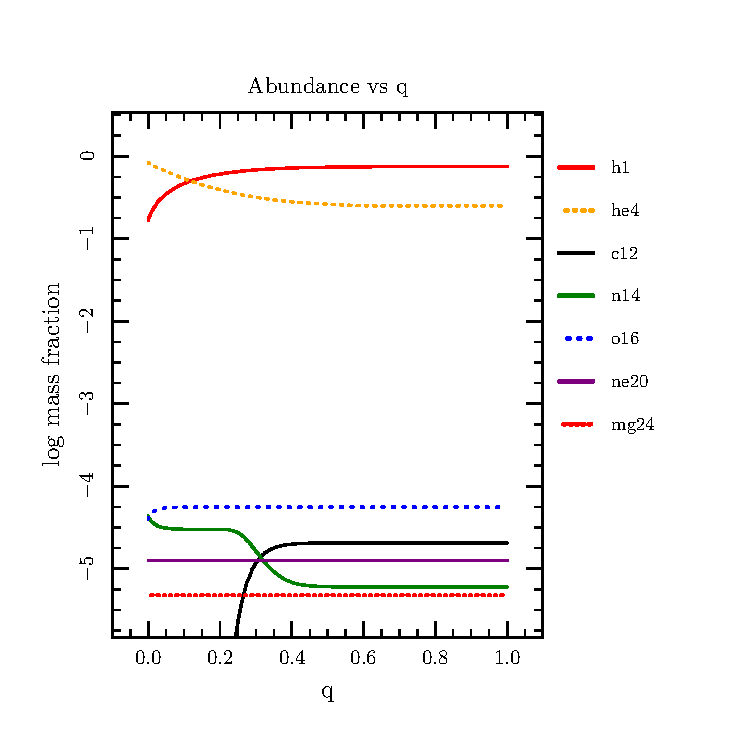
\includegraphics[width = 3.8in]{/Users/jaredbrooks/low_z/plots_out/Abundance_vs_q_22.pdf}
            \caption{Abundance profile at end of run}
            \label{fig:3}
          \end{minipage}
	\end{figure}

        \pagebreak

        The plot to the left (figure \ref{fig:5}) shows the evolution of star's radius.  To the right is a burning rate profile (figure \ref{fig:6}) from the end of the run.

        \begin{figure}[H]
          \begin{minipage}[b]{0.5\linewidth}
            \centering
            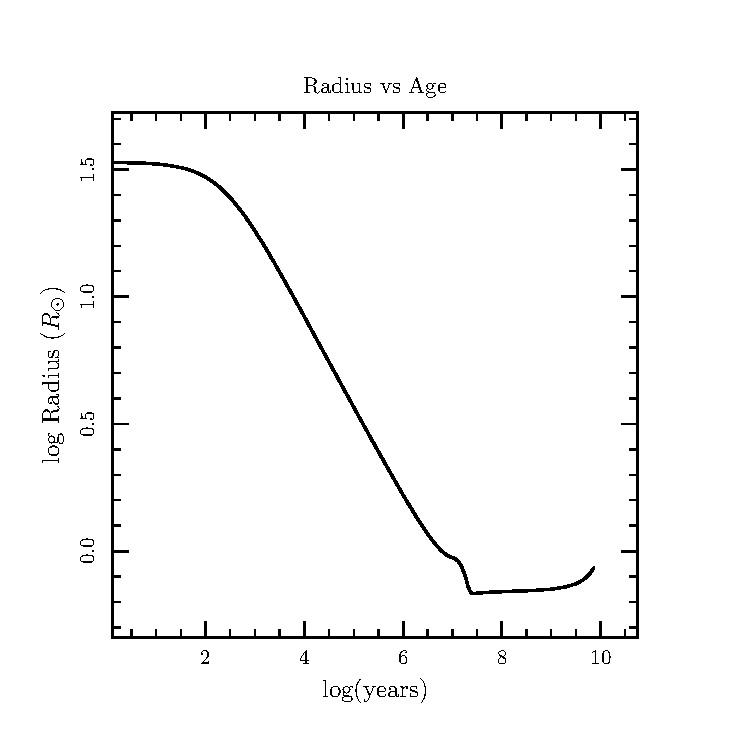
\includegraphics[width = 3.8in]{/Users/jaredbrooks/low_z/plots_out/Radius_vs_log_Age.pdf}
            \caption{Evolution of radius}
            \label{fig:5}
          \end{minipage}
          \hspace{0cm}
          \begin{minipage}[b]{0.5\linewidth}
            \centering
            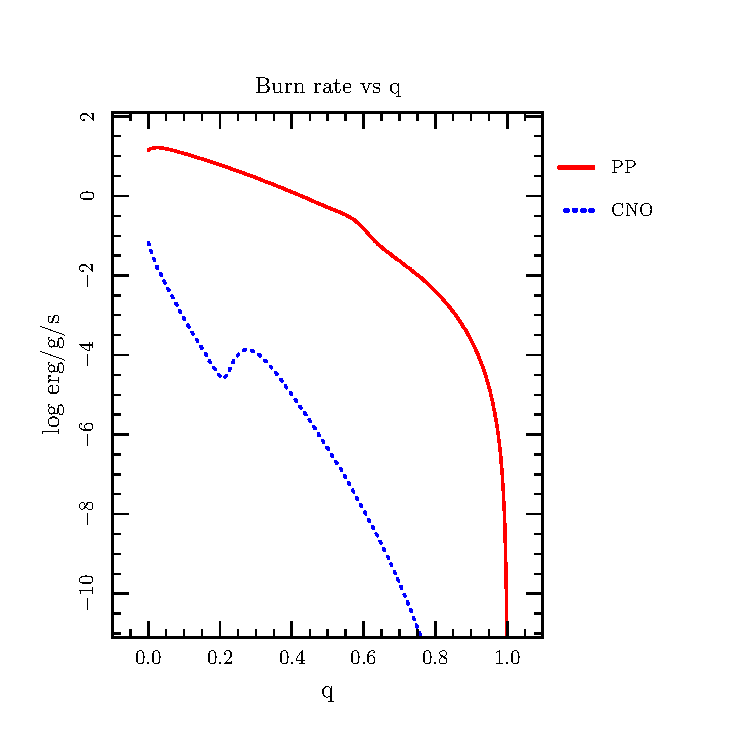
\includegraphics[width = 3.8in]{/Users/jaredbrooks/low_z/plots_out/Burnrate_vs_q_22.pdf}
            \caption{Burning rate profile from the end of the run}
            \label{fig:6}
          \end{minipage}
        \end{figure}

        \pagebreak

        This final plot (figure \ref{fig:7}) shows a few internal \texttt{MESA} variables, such as the size of the time-step, the number of zones, and the number of retries against the model number in order to give some understanding of how hard \texttt{MESA} is working throughout the run and where some areas of problems/interest might be.

        \begin{figure}[H]
          \centering
          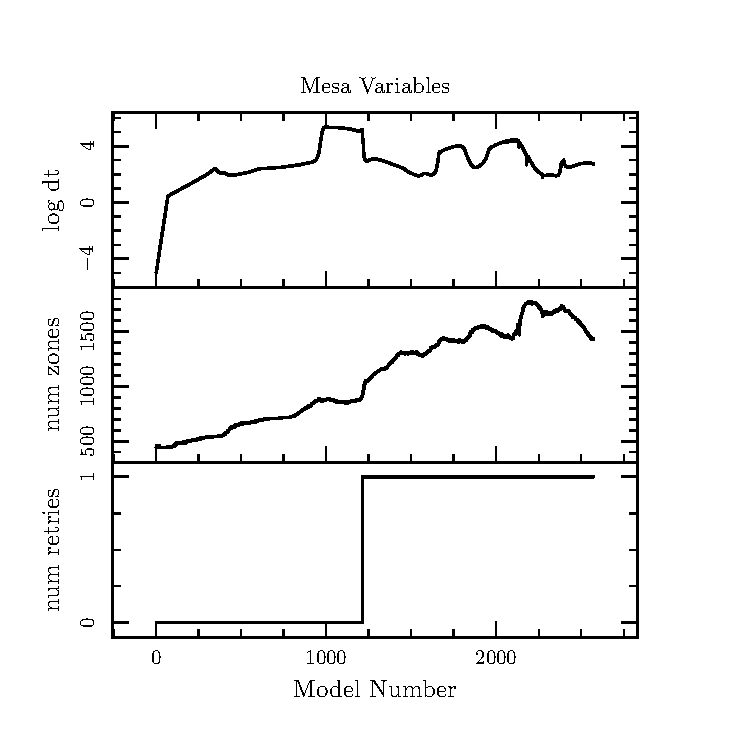
\includegraphics[width = 5in]{/Users/jaredbrooks/low_z/plots_out/Mesa_Variables.pdf}
          \caption{\texttt{MESA} variables plotted against model number show how hard \texttt{MESA} is working}
          \label{fig:7}
        \end{figure}

\end{document}
